%!TEX root = ../main.tex



\section{Preliminaries}\label{sec:preliminaries}
We employ standard terminology from (finite and classical) model theory~\cite[Sec. 1--3]{Libkin04}.

All the logics considered here will be fragments of the first-order logic ($\FO$) over purely-relational equality-free vocabularies, under the usual syntax and semantics. 
We fix a countably infinite set $\V \deff \{x_i \mid i \in \N\}$ of variables and a countably infinite set~$\R$ of predicates (we use $\arity(\relR)$ to denote the arity of $\relR$ from $\R$). 
Throughout this paper all the formulae will use only variables from $\V$ and predicates from $\R$.
Given a formula $\varphi$ we use $\sig(\varphi)$ we denote the set of predicates appearing in $\varphi$. 
We write $\varphi(\vartuplex)$ to indicate that all free variables from $\varphi$ are members of $\vartuplex$. 
If $\vartuplex$ contains precisely the free
variables of $\varphi$, then we will emphasise this separately.
A formula without free variables will be called a \emph{sentence}.
Given a structure $\str{A}$ and $B \subseteq A$, we will use $\restr{\str{A}}{B}$ to denote the \emph{substructure} of $\str{A}$ induced by $B$.\\

\noindent \textbf{Tuples and subsequences.}
An $n$-tuple is a sequence with $n$ elements. The $0$-tuple is denoted with $\emptytupl$.
We use $\vartuplexfromto{i}{j}$ to denote the $(j{-}i{+}1)$-tuple $\varx_i, \varx_{i+1}, \ldots, \varx_j$.
We say that $\vartuplexfromto{i}{j}$ is an infix of a tuple $\vartuplexfromto{k}{l}$ if $k \leq i \leq j \leq l$ holds. 
To improve readability, tuples of tuples will be denoted by arrows, for instance with $\elemtuptuplea$.
For a set $S$, we write $\vartuplex \sqin S$ iff $\varx_i \in S$ for all indices $1 \leq i \leq |\vartuplex|$, where $|\vartuplex|$ denotes the length of~$\vartuplex$. 
A tuple $\elemtuplea \sqin A$ is \emph{$\sigma$-live} (or simply \emph{live} if a signature $\sigma$ is known from the context) in $\str{A}$ if $|\elemtuplea| \leq 1$ or~$\elemtuplea \in \relR^{\str{A}}$ for some~$\relR \in \sigma$.\\

\noindent \textbf{Types and logical equivalence.}
Fix a logic $\logicL$, a finite signature~$\sigma \subseteq \R$. 
We~employ $\logicL[\sigma]$ in place of~$\{ \varphi \in \logicL \mid \sig(\varphi) \subseteq \sigma \}$.
Moreover, we use $\logicL_\ell[\sigma]$ to denote the restriction of $\logicL[\sigma]$ to formulae of quantifier rank (i.e.\ the maximal number of nested quantifiers) at most~$\ell$.  
%
The $\logicL[\sigma]$-type of $\elemtuplea$ in $\str{A}$, denoted with~$\tp{\logicL[\sigma]}{\str{A}}{\elemtuplea}$, consists of all $\logicL[\sigma]$-formulae with free variables~$\vartuplexfromto{1}{n}$ that are satisfied by $\elemtuplea$ in $\str{A}$.
We write $\str{A} \equiv_\logicL \str{B}$ if $\str{A}$ and $\str{B}$ satisfy the same $\logicL$-sentences.
For pointed structures $(\str{A}, \elemtuplea), (\str{B}, \elemtupleb)$ we use the notation $(\str{A}, \elemtuplea) \equiv_\logicL (\str{B}, \elemtupleb)$ to express that for all $\varphi \in \logicL$ with at most $\vartuplexfromto{1}{|\elemtuplea|}$ we have $\str{A} \models \varphi[\elemtuplea]$ if and only if $\str{B} \models \varphi[\elemtupleb]$ (variable $\varx_i$ is substituted with $\elemtuplea_i$). 
A similar notation is used for $\logicL[\sigma]$ instead of $\logicL$.\\

\noindent \textbf{Guarded fragments.}
We recall the definition of the \emph{guarded fragment}~\cite[Sec. 4.1]{AndrekaNB98}, \ie the fragment of $\FO$ obtained by requiring that blocks of quantifiers are appropriately relativised by atoms.
Formally $\GF$ is the smallest fragment of $\FO$  such that:
\begin{itemize}\itemsep0em
    \item Every atomic formula is in $\GF$;
    \item $\GF$ is closed under boolean connectives $\land, \lor, \neg, \to$;
    \item If $\varphi(\vartuplex, \vartupley)$ is in $\GF$ and $\alpha(\vartuplex, \vartupley)$ is an atom containing all free variables of $\varphi$ and $\vartupley$ is a tuple of variables then both $\forall{\vartupley} \; (\alpha(\vartuplex, \vartupley) \to \varphi(\vartuplex, \vartupley))$ and $\exists{\vartupley} \; (\alpha(\vartuplex, \vartupley) \land \varphi(\vartuplex, \vartupley))$ are in $\GF$; 
    \item If $\varphi(\varx)$ has only a single free-variable $\varx$, then $\forall{\varx}\; \varphi$ and $\exists{\varx}\; \varphi$ are in $\GF$.
\end{itemize}
The atoms $\alpha$ appearing in the 3rd item of the above definition are called \emph{guard}.
We stress that in definition of a quantifier rank for $\GF$ we count treat quantifiers $\exists{\vartuplex}$ introducing tuples of variables as as a single quantifier (not as an abbreviation for a block of quantifiers).

\begin{example}
  \begin{align*}
  \phi &= \exists{x_{1}x_{2}x_{3}} (\alpha(x_{1}, x_{2}, x_{3}) \and \forall x_{4}(\alpha(x_{4}, x_{4}, x_{1}) \to \alpha(x_{1}, x_{4}, x_{1}))) \in \GF \\
  \psi &= \exists{x_{1}x_{2}x_{3}} (E(x_{1}, x_{2}) \land E(x_{2}, x_{3}) \land E(x_{3}, x_{1})) \notin GF
  \end{align*}
\end{example}

The \emph{forward guarded fragment} $\FGF$~\cite[Sec. 3.1]{Bednarczyk21} restrict $\GF$ in a way that the allowed sequences of atoms are infixes of the sequence of already-introduced variables in the order of their quantification.
A formal definition comes next, which will be follow by a bunch of examples.
Let $\FGF(n)$ for $n \in \N$ be the smallest fragment of $\FO$ satisfying:
\begin{itemize}\itemsep0em
    \item An atom $\alpha(\vartuplex)$ belongs to $\FGF(n)$ if $\alpha$ is equality-free and $\vartuplex$ is an infix of $\vartuplexfromto{1}{n}$.
    \item $\FGF(n)$ is closed under boolean connectives $\land, \lor, \neg, \to, \iff$;
    \item If $\varphi$ is in $\FGF(n{+}k)$ for a positive $k$ and $\alpha(\vartuplex, \vartupley)$ is an atom containing all free variables of $\varphi$ and $\vartupley$ is a $k$-tuple of variables then  $\forall{\vartupley} \; (\alpha(\vartuplex, \vartupley) \to \varphi(\vartuplex, \vartupley))$ and $\exists{\vartupley} \; (\alpha(\vartuplex, \vartupley) \land \varphi(\vartuplex, \vartupley))$ are both in $\FGF(n)$; 
    \item If $\varphi(\varx_1) \in \FGF(1)$ has only a single free-variable $\varx_1$, then $\forall{\varx_1}\; \varphi$ and $\exists{\varx_1}\; \varphi$ are in $\FGF(0)$.
\end{itemize}
We use $\FGF$ to denote $\FGF(0)$. 
Note that $\FGF(0)$ is solely composed of sentences. 

\begin{example}
  \begin{align*}
    \phi_{1} &= \exists{x_1x_{2}x_{3}}(\alpha(x_{1}, x_{2}, x_{3}) \land \forall{x_{4}x_{5}}(\beta(x_{3}, x_{4}, x_{5}) \to \delta(x_{4})) \land \exists{x_{3}}(\gamma(x_{1}, x_{2}, x_{3}))) \in \FGF \\
    \phi_{2} &= \forall{x_{1}} (\alpha(x_{1}) \lor \beta(x_{1})) \in \FGF \\
    \phi_{3} &= \exists{x_{1}} E(x_{1}, x_{1}) \notin \FGF,\ \text{but} \in \GF \qquad \text{$x_1x_1$ is not an infix of $x_1$} \\
    \phi_{3} &= \exists{x_{1}} (\forall{x_{2}} \epsilon(x_{1}, x_{2})) \notin \FGF, \GF \qquad \text{$x_{1}, x_{2}$ is not guarded}
  \end{align*}
\end{example}

\noindent \textbf{Bisimulations for guarded fragments.}
%
We next present notion of bisimulation relations tailored towards $\GF$ and $\FGF$, based on presentations from~\cite[Sec. 2.2.3]{Otto04} and~\cite[Sec. 2]{BednarczykJ22}.

For a signature $\sigma \subseteq \R$ and $\sigma$-structures $\str{A}$ and $\str{B}$ we denote with $\PartIso{\str{A}}{\str{B}}$ the set of all partial isomorphisms between $\str{A}$ and $\str{B}$. 
For $\bisimZ, \bisimZ' \in \PartIso{\str{A}}{\str{B}}$ we say that $\bisimZ'$ satisfies back-and-forth conditions for $\bisimZ$ if for every partial isomorphism $\partisof \in \bisimZ$ we have:
%
\begin{description}\itemsep0em
  \item[\desclabel{(Forth)}{bisim:forth}] For any $\sigma$-live $\elemtuplea \sqin A$, there is $\partisog \in \bisimZ'$ with the domain $\elemtuplea$ such that $\partisof$ and $\partisog$ agree on their common domain. 
  \item[\desclabel{(Back)}{bisim:back}] For any $\sigma$-live $\elemtupleb \sqin B$, there is $\partisog \in \bisimZ'$ with the image $\elemtuplea$ such that $\partisof$ and $\partisog$ agree on their common domain. 
\end{description}
The set $\bisimZ$ is a $\GF[\sigma]$-\emph{bisimulation} between $\str{A}$ and $\str{B}$ if it itself satisfies \ref{bisim:forth} and~\ref{bisim:back} conditions given above and every partial isomorphism $\partisof \in \bisimZ$ maps $\sigma$-live tuples to $\sigma$-live tuples.
An $\ell$-$\GF[\sigma]$-bisimulation between $\str{A}$ and $\str{B}$ is a sequence $\bisimZ_0, \bisimZ_1, \ldots, \bisimZ_\ell$ of partial isomorphisms from $\PartIso{\str{A}}{\str{B}}$ mapping $\sigma$-live tuples to $\sigma$-live tuples  such that for all $i > 0$ we have that $\bisimZ_i$ satisfies~\ref{bisim:forth} and~\ref{bisim:back} conditions for $\bisimZ_{i{-}1}$.
We say that pointed structures $(\str{A}, \elemtuplea)$ and~$(\str{B}, \elemtupleb)$ are $\GF[\sigma]$-\emph{bisimilar}, denoted $(\str{A}, \elemtuplea) \bisimto_{\GF[\sigma]} (\str{B}, \elemtupleb)$ if there exists a $\GF[\sigma]$-bisimulation  between $\str{A}$ and $\str{B}$ containing the partial isomorphism $\elemtuplea \mapsto \elemtupleb$.
We analogously speak about $\ell$-$\GF[\sigma]$-\emph{bisimilarity} and employ the notation $(\str{A}, \elemtuplea) \bisimto_{\GF[\sigma]}^{\ell} (\str{B}, \elemtupleb)$.

The following classical lemma links bisimulations and logical~equivalence.
\begin{lemma}[Thm. 1.12 of~\cite{Gradel014}]\label{lemma:GF-bisimulations-work-well}
For any finite signature $\sigma$ and $\sigma$-structures $(\str{A}, \elemtuplea)$ and~$(\str{B}, \elemtupleb)$:
\begin{enumerate}[(a)]
\item $(\str{A}, \elemtuplea) \bisimto_{\GF[\sigma]} (\str{B}, \elemtupleb)$ implies $(\str{A}, \elemtuplea) \equiv_{\GF[\sigma]} (\str{B}, \elemtupleb)$;
\item $(\str{A}, \elemtuplea) \bisimto_{\GF[\sigma]}^{\ell} (\str{B}, \elemtupleb)$ implies $(\str{A}, \elemtuplea) \equiv_{\GF_\ell[\sigma]} (\str{B}, \elemtupleb)$;
\end{enumerate}
Moreover, the converse holds for $\omega$-saturated $\str{A}$ and $\str{B}$.
\end{lemma}

The following example presents two structures that are $\GF$-bisimilar but can be distinguished by a first-order formula.
\begin{example}
  Let $\phi = \exists{x_{1}, x_{2}, x_{3}}(E(x_{1}, x_{2}) \land E(x_{2}, x_{3}) \land E(x_{3}, x_{1}))$. Then $\str{A} \models \phi$ but $\str{B} \not\models \phi$, for the structures:
  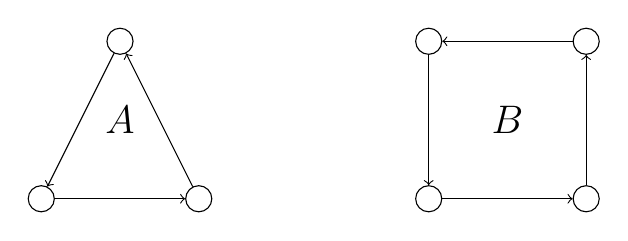
\begin{tikzpicture}[every node/.style={draw,circle}, baseline=(current bounding box.north)]
    \begin{scope}[xshift=-70]
    \node[draw=none, font=\Large] {$\str{A}$};
    \path[->]
      (1,-1) node(n1) {}
      (0,1) node(n2) {}
      (-1,-1) node(n3) {}
      (n1) edge (n2)
      (n2) edge (n3)
      (n3) edge (n1);
    \end{scope}

    \node[draw=none, font=\Large] {$\bisimto_{\GF}$};

    \begin{scope}[xshift=70]
    \node[draw=none, font=\Large] {$\str{B}$};
    \path[->]
      (1,-1) node(n1) {}
      (1,1) node(n2) {}
      (-1,1) node(n3) {}
      (-1,-1) node(n4) {}
      (n1) edge (n2)
      (n2) edge (n3)
      (n3) edge (n4)
      (n4) edge (n1);
    \end{scope}
  \end{tikzpicture}

\end{example}

Now a similar characterisation can be provided for $\FGF$. 
Due to the ``forwardness'' of the underlying logic, it is convenient to think about maps as tuples.
A \emph{system of forward partial maps} between $\sigma$-structures $\str{A}$ and $\str{B}$ is any non-empty subset of $\bigcup_{i=0}^{\infty} (A^i \times B^i)$ satisfying:
\begin{description}\itemsep0em
  \item[\desclabel{(AtomicEq)}{bisim:atomiceq}] For all $(\elemtuplea, \elemtupleb) \in \bisimZ$ we have that $\elemtuplea$, $\elemtupleb$ are $\sigma$-live and $\tp{\FGF[\sigma]}{\str{A}}{\elemtuplea} = \tp{\FGF[\sigma]}{\str{B}}{\elemtupleb}$~holds.
\end{description}
If $\bisimZ, \bisimZ'$ are systems of forward partial maps between $\str{A}$ and $\str{B}$, we say that $\bisimZ'$ satisfies back-and-forth conditions for $\bisimZ$ if for every $(\elemtuplea, \elemtupleb) \in \bisimZ$ the following conditions hold:
\begin{description}\itemsep0em
  \item[\desclabel{(fForth)}{bisim:fforth}] For a (possibly empty) affix $\elemtuplecfromto{i}{j}$ of $\elemtuplec$ and a $\sigma$-live tuple $\elemtuplee$ in $\str{A}$ such that $\elemtuplecfromto{i}{j} = \elemtupleefromto{1}{j{-}i{+}1}$ there is a $\sigma$-live tuple $\elemtuplef$ with $\elemtupledfromto{i}{j} = \elemtupleffromto{1}{j{-}i{+}1}$ such that $(\elemtuplee, \elemtuplef) \in \bisimZ$ holds.
  %
  \item[\desclabel{(fBack)}{bisim:fback}] For a (possibly empty) affix $\elemtupledfromto{i}{j}$ of $\elemtupled$ and a $\sigma$-live tuple $\elemtuplef$ in $\str{B}$ such that $\elemtupledfromto{i}{j} = \elemtupleffromto{1}{j{-}i{+}1}$ there is a $\sigma$-live tuple $\elemtuplee$ with $\elemtuplecfromto{i}{j} = \elemtupleefromto{1}{j{-}i{+}1}$ such that $(\elemtuplee, \elemtuplef) \in \bisimZ$ holds.
\end{description}
A system of forward partial maps $\bisimZ$ between $\str{A}$ and $\str{B}$ is a $\FGF[\sigma]$-\emph{bisimulation} between $\str{A}$ and $\str{B}$ if it itself satisfies the above conditions. 
An $\ell$-$\FGF[\sigma]$-bisimulation between $\str{A}$ and $\str{B}$ is a sequence $\bisimZ_0, \bisimZ_1, \ldots, \bisimZ_\ell$ of systems of forward partial maps between $\str{A}$ and $\str{B}$ such that for all $i > 0$ we have that $\bisimZ_i$ satisfies~\ref{bisim:fforth} and~\ref{bisim:fback} conditions for $\bisimZ_{i{-}1}$.
We speak about $\FGF[\sigma]$-\emph{bisimilar} and $\ell$-$\FGF[\sigma]$-\emph{bisimilar} (pointed) structures in total analogy to the case of the guarded fragment.
A ``forward'' counterpart of \cref{lemma:GF-bisimulations-work-well} is presented below.
\begin{lemma}\label{lemma:FGF-bisimulations-work-well}
For any finite signature $\sigma$ and $\sigma$-structures $(\str{A}, \elemtuplea)$ and~$(\str{B}, \elemtupleb)$:
\begin{enumerate}[(a)]
\item $(\str{A}, \elemtuplea) \bisimto_{\FGF[\sigma]} (\str{B}, \elemtupleb)$ implies $(\str{A}, \elemtuplea) \equiv_{\FGF[\sigma]} (\str{B}, \elemtupleb)$;
\item $(\str{A}, \elemtuplea) \bisimto_{\FGF[\sigma]}^{\ell} (\str{B}, \elemtupleb)$ implies $(\str{A}, \elemtuplea) \equiv_{\FGF_\ell[\sigma]} (\str{B}, \elemtupleb)$;
\end{enumerate}
Moreover, the converse holds for $\omega$-saturated $\str{A}$ and $\str{B}$.
\end{lemma}
\begin{proof}
  We show ``(b)'' analogously to the proof of ``(a)'' found in~\cite[appendix]{BednarczykJ22}.

  For the ``$\implies$'' direction, first consider quantifier-free (quantifier rank zero) formulae.
  If $\str{A}, \elemtuplea \bisimto_{\FGF[\sigma]}^{\ell} \str{B}, \elemtupleb$ then $\elemtuplea$ and $\elemtupleb$ must have equal forward types by \ref{bisim:atomiceq}.
  This means that they satisfy the same atomic formulae.
  By structural induction, this also holds for boolean combinations of formulae.
  Therefore, $\str{A}, \elemtuplea$ and $\str{B}, \elemtupleb$ satisfy the same quantifier-free FGF-formulae.

  Now by strong induction, let $\phi(x_{1}, \ldots, x_{n})$ be a FGF-formulae and assume the lemma is true for all $\ell$ less than the quantifier rank of $\phi$.
  By symmetry, assume w.l.o.g. $\str{A}, (a_{1}, \ldots, a_{n}) \models \phi$.

  Consider the case where $\phi(x_{1}, \ldots, x_{n}) = \exists{x_{(n+1)}\cdots{}x_{m}} \alpha(x_{i}, \ldots, x_{j}) \land \psi(x_{i}, \ldots, x_{j})$ ($\alpha$ is the atomic guard).
  Let $\ell$ be the quantifier rank of $\phi$, then $\alpha(x_{i},\ldots,x_{j}) \land \psi(x_{i}, x_{j})$ has quantifier rank $\ell - 1$.
  Thus there exist $a_{n+1}, \ldots, a_{j}$ such that $\str{A} \models \alpha(a_{i}, \ldots, a_{j}) \land \psi(a_{i}, \ldots, a_{j})$.
  As $(a_{i}, \ldots, a_{j})$ is guarded by $\alpha$, we can apply~\ref{bisim:fforth} to find $b_{n+1}, b_{j}$ with $\str{A}, (a_{i}, \ldots, a_{j}) \sim_{\FGF}^{\ell-1} \str{B}, (b_{i}, \ldots, b_{j})$.
  By the induction hypothesis, $\str{B}, (b_{i}, \ldots, b_{j}) \models \alpha(b_{i}, \ldots, b_{j}) \land \psi(b_{i}, \ldots, b_{j})$ and therefore also $\str{B}, (b_{1}, \ldots, b_{n}) \models \phi$.

  For the case that $\phi = \exists{x_{1}} \psi(x_{1})$, we know that $\str{A}, a_{1} \models \psi$.
  \possiblelie{Because the bisimulation must map every element to some element}, there must be $b_{1}$ with $\str{A}, a_{1} \bisimto_{\FGF}^{\ell-1} \str{B}, b_{1}$.
  Since $\psi$ has quantifier rank $\ell - 1$ we get $\str{B}, b_{1} \models \psi$ by the induction hypothesis and therefore also $\str{B} \models \phi$ as wanted.

  Again, we have that the above also holds for all boolean combinations of formulae as the lemma is preserved under boolean combinations.
  As $\forall{\bar{x}} \alpha(\bar{x}) \rightarrow \psi(\bar{x}) = \neg \exists{\bar{x}} \alpha(\bar{x}) \land \neg \psi(\bar{x})$, this also handles the case of universal quantification.

  For the converse, we show that the sets $Z_{0}, \ldots, Z_{\ell}$ defined as follows are a system of forward partial maps obeying the laws of a $\ell$-$\FGF$-bisimulation:
  \begin{equation*}
  \mathcal{Z}_{k} = \left\{ (\elemtuplea, \elemtupleb) \in \bigcup_{n < \omega} (A^{n} \times B^{n}) \mid \str{A}, \elemtuplea \equiv_{\FGF_{k}} \str{B},\elemtupleb \right\}
  \end{equation*}
  Each $Z_{k}$ satisfies~\ref{bisim:atomiceq} as $\str{A}, \elemtuplea \equiv_{\FGF_{k}} \str{B},\elemtupleb$ implies that $\elemtuplea$ and $\elemtupleb$ satisfy the same atomic formulae.

  To show~\ref{bisim:fforth} (\ref{bisim:fback} is symmetric), let $(\elemtuplea, \elemtupleb) \in Z_{k}$ and $\elemtuplec = \elemtuplea_{i\ldots{}j}\elemtuplee$ be a live tuple in $\str{A}$.
  Consider the $|e|$-type (over $\elemtupleb_{i\ldots{}j}$) of all tuples $\bar{f}$ for which $\str{A}, \elemtuplea_{i\ldots{}j}\elemtuplee \equiv_{\FGF}^{k-1} \str{B}, \elemtupleb_{i\ldots{j}}\bar{f}$:
  \begin{align*}
    \Sigma^{\elemtupleb_{i\ldots{j}}}(\bar{f}) = \left\{ \phi(\elemtupleb_{i\ldots{}j}\bar{f}) \mid \phi(\bar{x}) \in {\FGF(|c|)_{k-1}}\ \text{and}\ \str{A}, \elemtuplec \models \phi(\bar{x}) \right\}
  \end{align*}
  We claim that $\Sigma^{\elemtupleb_{i\ldots{}j}}(\bar{f})$ is realized in $\str{B}$.
  By $\omega$-saturation and compactness it suffices to show that it is finitely satisfiable in $\str{B}$.
  Let $\Delta \subseteq \Sigma^{\elemtupleb_{i\ldots{}j}}(\bar{f})$ be a finite subset.
  Then $\delta(\bar{x}_{i\ldots{}i+|c|}) = \bigwedge \Delta[\elemtupleb_{i\ldots{}j} \mapsto \bar{x}_{i\ldots{}j}, \bar{f} \mapsto \bar{x}_{(j+1)\ldots{}(j+|e|)}]$ is a $\mathrm{FGF}_{k-1}$ formula.
  Since $\elemtuplec$ is live, there must a relation $\alpha$ such that $\elemtuplea, \elemtuplec \models \alpha(x_{1\ldots{}|c|})$.
  We can now construct the $\mathrm{FGF}_{k}$-formula $\chi = \exists{x_{j+1}\cdots{}x_{j+|e|}} (\alpha(x_{i\ldots{}i+|c|}) \land \delta(\bar{x}_{i\ldots{}i+|c|}))$.
  We have $\str{A}, \elemtuplea \models \chi$ (witnessed by $\elemtuplee$) and thus also $\str{B}, \elemtupleb \models \chi$ as they satisfy the same $\mathrm{FGF}_{k}$ formulae by assumption.
  So there must be $\bar{f}$ satisfying $\str{B}, \elemtupleb_{i\ldots{}j}\bar{f} \models \delta(\bar{x}_{i\ldots{}i+|c|})$, which by construction means that $\str{B}, \bar{f} \models \Delta$.
\end{proof}

The following example presents two structures that are $\FGF$-bisimilar but not $\GF$-bisimilar.
\begin{example} Let $\phi = \exists{x_{1}} E(x_{1}, x_{1})$. Consider the structures
  $\str{A}$ (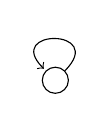
\begin{tikzpicture}[baseline=(n1.base), trim left=-10pt, trim right=10pt] \node[draw,circle] (n1) {}; \draw[->] (n1) edge[loop] (n1); \end{tikzpicture}) and
  $\str{B}$~(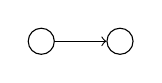
\begin{tikzpicture}[baseline=-3pt] \node[draw,circle] (n1) {}; \node[draw,circle] (n2) at (1,0) {}; \draw[->] (n1) edge (n2); \end{tikzpicture}).
  There is a $\FGF$-bisimulation between $\str{A}$ and $\str{B}$ which maps every element of $\str{B}$ to the single element in $\str{A}$.
  But $\str{A} \not\bisimto_{\GF} \str{B}$ as they can be distinguished by the $\GF$-sentence $\phi = \exists{x_{1}} E(x_{1}, x_{1})$: $\str{A} \models \phi$ and $\str{B} \not\models \phi$.
\end{example}
